\chapter{Proposta de Classificação}
A classificação de recursos facilitará o desenvolvimento de novos \emph{drivers} para futuras aplicações, pois possibilitará a definição de interfaces pré-estabelecidas que representem classes de recursos. Outra vantagem decorrente é a possibilidade de seleção de recursos equivalentes, caso o provedor originalmente selecionado esteja indisponível.

Após pesquisas, estudos e comparações realizadas e apresentadas em seções anteriores, propõe-se uma classificação que seja relacionada, extensível, que permita a um recurso pertencer à multiplas classes simultaneamente e cuja representação seja via JSON (\emph{JavaScript Object Notation}).

\begin{comment}
Neste capítulo falaremos sobre a classificação de dispositivos proposta. Essa classificação deverá ser relacionada, extensível e um dispositivo deverá poder fazer parte de múltiplas classes. A classificação relacionada facilita a implementação de novos \emph{drivers} para o \emph{uOS} que poderão se aproveitar das interfaces já existentes. Ser extensível, pois permite uma relação de especialização entre diferentes classes. A capacidade de permitir que um dispositivo pertença à diferentes classes, garante uma flexibilidade para dispositivos com diversos recursos poderem se encaixar nas classificações padrões sem a necessidade da definição de uma nova classe.
\end{comment}

\begin{itemize}
	\item Forma de classificação

	Optou-se por uma classificação relacionada, em que classes de recursos podem se relacionar umas com as outras utilizando-se herança ou composição. A primeira possibilita a extensão, em que interfaces previamente estabelecidas seriam utilizadas na elaboração de novos \emph{drivers}. Obtêm-se, com isso, a possibilidade da utilização de polimorfismo e a vantagem de que cada classe represente exatamente um objeto tão simples quanto possível, almejando-se obter uma alta coesão e um baixo acoplamento. A segunda permite que uma classe contenha, em sua definição, zero ou mais classes. Dessa forma, torna-se possível a delegação de responsabilidades para serviços existentes em outras classes outrora estabelecidas, evitando tanto a repetição de código como um alto acoplamento.

	\item Representação

	Em um ambiente cujos dispositivos podem se movimentar livremente e seus recursos devem ser compartilhados de forma transparente ao usuário, torna-se necessário que cada dispositivo presente na rede possa se comunicar facilmente com os demais. Atualmente, o \emph{uOS} já utiliza JSON em suas trocas de mensagens e substituí-lo seria inviável.

	\begin{comment}
	Tal formato apresenta as seguintes características:
	
		\begin{itemize}
	 		\item Baixo custo computacional~\cite{comparativojson};
	 		\item É auto-descritivo, o que facilita os processos de leitura e escrita por seres-humanos~\cite{json};
	 		\item É estruturado, o que facilita sua criação e análise por computadores~\cite{json};
	 		\item É independente de plataforma, pois utiliza UTF-8 como codificação~\cite{utf8}.
	 	\end{itemize}
	 \end{comment}
\end{itemize}

\section{A Classificação}
Levando-se em consideração os fatores apresentados anteriormente e analisando-se a tabela~\ref{tab:comparativoClasses}, definiu-se as seguintes classes padrões:

\begin{itemize}
	\item Cliente de Áudio
		
		Abrange quaisquer tipos de dispositivos que contenham a capacidade de reproduzir áudio Exemplo: TVs, celulares, aparelhos de som;
	\item Servidor de Áudio
		
		Abrange quaisquer tipos de dispositivos que possam operar como servidor de áudio Exemplo: TVs, celulares, aparelhos de som;
	\item Cliente de Vídeo
		
		Abrange quaisquer tipos de dispositivos que possuam a capacidade de prover um recurso de renderização de vídeo. Exemplo: TVs, celulares, projetores;
	\item Servidor de Vídeo
		
		Abrange quaisquer tipos de dispositivos que possuam operar como servidor de vídeo. Exemplo: TVs, celulares;
	\item Display de Imagem
		
		Abrange quaisquer tipos de dispositivos que possam prover um recurso de renderização de imagem. Exemplo: TVs, celular, impressora;
	\item Servidor Imagem
		
		Abrange quaisquer tipos de dispositivos que possam operar como servidor de imagem. Exemplo: câmeras digitais, \emph{scanners};
	\item Teclado
		
		Abrange quaisquer tipos de dispositivos que possam prover um recurso de teclado. Exemplo: teclados, \emph{notebooks}, celulares, \emph{tablets};
	\item Apontador
		
		Abrange quaisquer tipos de dispositivos que possuam o recurso de apontadores. Exemplo: \emph{mouses}, telas sensíveis ao toque, \emph{joysticks};
\end{itemize}

Tal definição é importante pois é ela que permitirá um agrupamento de recursos em torno de suas funcionalidades, a saber, os seus serviços. Seu valor ficará mais claro com a leitura das próximas seções, nas quais os conceitos de ``Equivalência de recursos" e ``Árvore de Equivalência" serão apresentados.

\begin{comment}
Suponha que um usuário, por meio de uma aplicação de seu celular, deseja utilizar os serviços providos de um recurso de imagem. Considere ainda, que existam três instâncias disponíveis deste recurso no \emph{smart space}. Para garantir a equivalência dos recursos devemos garantir que eles possuam os mesmos serviços, e para isso, devemos garantir que os serviços possuam a mesma interface, ou seja, os mesmos tipos e número de parâmetros. Suponha que para o usuário que deseja o recurso simples de imagem seja indiferente a quantidade de \emph{megapixels} da imagem. Para o usuário basta apenas o provimento do serviço que retorne algum dado ou altere o estado de alguma aplicação. Dessa forma, devemos garantir que qualquer uma das três instâncias possam prover esse serviço. Uma câmera com \emph{flash}, por exemplo, para este cenário, seria equivalente a um recurso de câmera sem \emph{flash}.
\end{comment}

\section{Equivalência de Recursos}
\label{sec:equivalenciaRecursos}

Entende-se por equivalência tudo aquilo que tem o mesmo valor.

\begin{quote}
	Lucas estava brincando com seu carrinho, quando uma das rodinhas se quebrou. Entristecido, ele procurou por seu pai, que, ao ver a aflição de seu filho, resolveu ajudar. Recolheu uma garrafa PET que estava por perto, desenroscou sua tampinha e a colocou no lugar deixado pela rodinha estragada. Tamanha foi a felicidade de Lucas ao poder voltar a brincar com o seu carrinho.
\end{quote}

A história acima, apesar de simples, contém informações que podem ser úteis. Observe que os objetos envolvidos, ou seja, a rodinha e a tampinha, diferem na maioria das suas características: material, valor, peso, cor, etc. Entretanto, apesar de tudo, pelo menos uma das características é igual: ambas possuem formatos cilíndricos. Foi essa única semelhança que permitiu o conserto do carrinho e garantiu a felicidade de Lucas! Ou seja, no contexto apresentado, a rodinha e a tampinha puderam ser trocadas sem perda de valor.

É exatamente esse o sentido ao se afirmar que dois recursos são equivalentes. Um não precisa ser igual ao outro, mas apenas possuir uma característica que, em determinado momento, possibilite a intercambialidade. Seria possível, por exemplo, utilizar um \emph{joystick} como um dispositivo apontador e, a qualquer momento, substitui-lo por um \emph{laser pointer} de forma que os serviços necessários continuassem sendo providos. Repare que tais dispositivos, assim como a rodinha e a tampinha, são bastante diferentes em diversas de suas características, mas ainda assim são capazes de fornecer serviços iguais, como mover uma seta pela tela.

\subsection{Cálculo de Equivalência}

Para que um recurso R1 seja equivalente a um recurso R2, os serviços de R2 deverão estar presentes no conjunto de serviços de R1, mas R1 poderá ter outros serviços que não estão presentes em R2. Seja S(X), o conjunto de serviços do recurso X, então teríamos que $S(R1) \cap S(R2) = S(R2)$. 

\begin{figure}[ht]
	\center
	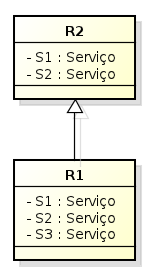
\includegraphics[scale=0.6]{imagens/equivalenciaDeRecursos}
	\caption{Exemplo de recursos equivalentes.}
	\label{fig:equivalenciaDeRecursos}
\end{figure}

Suponha uma situação em que $A \implies B$, $B \implies C$ e $C \implies A$, logo teríamos que $A \implies C$, o que seria uma relação circular, o que não faz sentido, pois concluiríamos que todos os recursos são iguais e não equivalentes. Devemos, portanto, garantir que não ocorra essa equivalência circular. Caso algum dispositivo queira registrar um novo \emph{driver} que cause essa inconsistência, devemos impedir que essa inconsistência possa ocorrer, ou então alertar o novo driver da ocorrência deste problema e não realizar seu registro. 

\subsection{Consistência de Interface}

	A figura~\ref{fig:consistenciaInterface} mostra que o recurso R1 é equivalente ao recurso R3, mas embora possua um serviço de mesmo nome que o recurso R2,  seus parâmetros são diferentes, logo, não pode ser um mesmo serviço e os recursos não serão equivalentes..
	
	Para garantir que os recursos são equivalentes, devemos realizar três validações nas interfaces de cada serviço dos recursos:
	\begin{enumerate}
		\item Recurso:
			
			Os serviços devem pertencer ao mesmo recurso cujas classes padrões foram definidas anteriormente.
		
		\item Identificador do Serviço:

			Os serviços devem possuir os mesmos identificadores.

		\item Parâmetros:

			Os serviços devem possuir os mesmos parâmetros.
	\end{enumerate}

	Parte-se do princípio que não existirá interesse em camuflar um serviço malicioso ao expor uma interface compatível com a equivalência.

\begin{figure}[ht]
	\center
	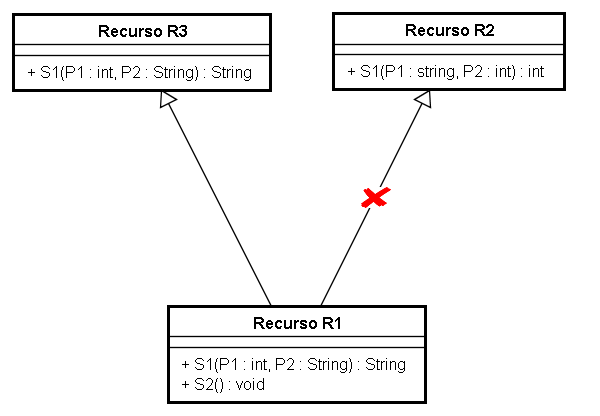
\includegraphics[scale=0.8]{imagens/consistenciaInterface}
	\caption{Exemplo de inconsistência de interface.}
	\label{fig:consistenciaInterface}
\end{figure}

\begin{comment}
----------------------------------------- REVER ----------------------------------------- \\
Desta forma, faz-se necessária uma maneira de classificar tais recursos imersos nos mais variados dispositivos presentes no \emph{smart space} e regidos pelo \emph{middleware}. Essa classificação facilitará o desenvolvimento de novos \emph{drivers} para futuras aplicações, pois tornará possivel a definição de interfaces pré-estabelecidas que representem classes de recursos. Outra vantagem decorrente é a possibilidade de seleção de recursos equivalentes, caso o provedor originalmente selecionado esteja indisponível. \\
----------------------------------------- REVER -----------------------------------------

COLOQUEI NO COMEÇO DA PROPOSTA
\end{comment}

\section{Impacto}
\label{sec:impactoUOS}

A proposta anteriomente definida requer algumas mudanças no \emph{uOS}. Esta seção mostrará um pouco mais sobre como o \emph{uP} foi definido a partir dos conceitos da DSOA e, por fim, mostrará os impactos do uso da classificação para a determinação da equivalência de recursos.

O \emph{uP (Ubiquitous Protocols)} foi construído baseado na arquitetura DSOA. É um conjunto de protocolos criado com objetivo de estabelecer um meio de interação entre os serviços dentro desta arquitetura. Tais protocolos definem o canal de comunicação e a forma de interação entre as entidades do ambiente. As mensagens são transmitidas no formato JSON (\emph{JavaScript Object Notation})~\cite{json}.

\begin{comment}
, que utiliza a codificação UTF-8~\cite{utf8}, que foi escolhido por ser um formato estruturado, leve e independente de plataforma. O JSON foi utilizado ante o XML, pois possui menor tamanho de mensagens e esse fator pode ser decisivo em um ambiente com diversos dipositivos com capacidades computacionais diferentes e possivelmente reduzidas. Dessa forma a limitação dos dispositivos é minimizada e exclui a necessidade de uma rede para tratamento dessas mensagens.
\end{comment}

Cada um dos conceitos apresentados na DSOA possui uma representação no \emph{uP} com seus respectivos atributos:

\begin{itemize}
	\item Dispositivo(\emph{UpDevice}):
	
		Por meio dos seguintes atributos, é possível identificar unicamente o dispositivo no ambiente, e quais são as interfaces rede que o dispositivo possui para realizar alguma comunicação:

	\item \emph{Driver}(\emph{UpDriver}): 

		Representa o conceito do Recurso definido na DSOA. Como um dispositivo pode ter várias instâncias de um recurso, cada instância é identificada unicamente dentro do dispositivo que contém este recurso.

	\item Serviço(\emph{UpService}): 

		Representa o conceito de mesmo nome definido na DSOA.
\end{itemize}

Além disso, com o objetivo de disponibilizar as características de visibilidade, interação e efeito, foram criados mecanismos de acesso aos recursos. O \emph{uP} é dividido em protocolos básicos, que são utilizados para invocar serviços e protocolos complementares que completam suas funcionalidades.

\begin{itemize}
	\item Protocolos Básicos: 

		São divididos em SCP (\emph{Service Call Protocol}) e EVP(\emph{Event Protocol}). O primeiro possui arquitetura provedor-consumidor, ou seja, o consumidor requisita um serviço e o provedor retorna esse serviço para ele de forma síncrona. No último, o consumidor se registra em um evento no provedor, que response informando que o registro foi realizado com sucesso, e na ocorrência do evento, o consumidor é notificado pelo provedor, demonstrando uma forma assíncrona de comunicação.
	\item Protocolos Complementares:

		Além da interação entre os serviços provida pelos protocolos básicos, o \emph{uP} tem mecanismos que permitem que as aplicações obtenham informações sobre quais são os serviços disponíveis no ambiente e informações a respeito deles. Os protocolos são divididos em um grupo de protocolos com informações sobre o dispositivo e um grupo de protocolos com informações sobre o ambiente. 
\end{itemize}

O conceito do Recurso introduzido anteriormente na subseção~\ref{subsec:introUos} do capítulo~\ref{cap:classificacao} será afetado devido a proposta de classificação de recursos. Um dispositivo presente no \emph{smart space}, segundo a DSOA, procura seus serviços no ambiente por meio do identificador do recurso que provê esses serviços. Com a introdução do conceito de Equivalência de Recursos, o dispositivo irá procurar por uma classe desse recurso. O identificador, em vez de representar um nome do recurso, irá, portanto, identificar que tipo de recurso ele representa, ou seja, recurso de: imagem, áudio, apontador e etc. Na visão da DSOA, a interface do recurso foi acrescida da lista de recursos equivalentes. Dessa forma, o recurso fica responsável por informar os recursos aos quais ele é diretamente equivalente. Por exemplo, se $R1 \implies R2$, $R1 \implies R3$ e $R3 \implies R4$, então o recurso $R1$ irá informar que ele é equivalente a $R2$ e $R3$ apenas.

Como \emph{uP} foi criado a partir dos conceitos da DSOA, o impacto sofrido na DSOA foi diretamente refletido sobre ele. Para que a equivalência de serviços possa ser garantida, os recursos do dispositivo, cada um representado por um \emph{UpDriver}, deverá informar os recursos aos quais este é equivalente. Além disso, o identificador do recurso representará a classe deste. Dessa forma, a interface do recurso foi acrescida de um campo para informar estes \emph{drivers}. O \emph{UpDriver} ficará, portanto, com os seguintes campos:

\begin{itemize}
	\item \emph{``name''}:
		
		Representa a classe do recurso.

	\item \emph{``equivalentDrivers''}:
	
		Classes a que este recurso é equivalente.
	\item \emph{``services''}:

		Lista dos serviços síncronos do recurso.

	\item \emph{``events''}:

		Lista dos serviços assíncronos do recurso;
\end{itemize}

O campo \emph{``equivalentDrivers''} irá carregar a informação sobre a equivalência de um recurso. Entretanto, em um ambiente dinâmico, existe a possibilidade do \emph{uOS} não conhecer um destes recursos equivalentes. O dispositivo, então, ficará responsável por prover um serviço que informe ao \emph{uOS} a interface deste(s) recurso(s) desconhecido(s) e sua(s) equivalência(s) até a raiz conhecida pelo \emph{uOS}, para que o \emph{middleware} possa encontrar e registrar este novo driver na árvore de recursos. Para isso, deverá ser criado mais um serviço no protocolo \emph{Device Driver}, um dos protocolos complementares do \emph{uP}, que ficará com os seguintes serviços:

\begin{itemize}
	\item \emph{ListDrivers}: 

		Provê uma lista de instâncias dos drivers disponíveis do dispositivo. Possui dois parâmetros opcionais:
		\begin{itemize}
			\item \emph{``serviceName''}: 

				Nome do serviço;
			\item \emph{``driverName''}: 

				Identificador do recurso.
		\end{itemize}
	\item \emph{Handshake}: 

		Neste protocolo, dois dispositivos trocam informações entre-si. O dispositivo que invoca esse serviço passa como parâmetro um objeto do tipo \emph{device} e recebe como retorno informações sobre o dispositivo que recebeu a chamada;
	\item \emph{Goodbye}: 

		Responsável por retirar o dispositivo da lista de dispositivos presentes no ambiente;
	\item \emph{Authenticate}: 

		Estabelece um contexto de segurança entre dois dispositivos por meio de um prévio compartilhamento de chaves.

	\item \emph{TellEquivalentDrivers}:

		Responsável por informar a interface do(s) recurso(s) desconhecido(s) equivalente(s). Será composto pelos seguintes campos:

		\begin{itemize}
			\item \emph{``driversName''}:

			Lista com o(s) nome(s) do(s) recurso(s).

			\item \emph{``interfaces''}:

			Lista com a(s) interface(s) do(s) recurso(s).
		\end{itemize}
\end{itemize}


\begin{comment}
Serão afetados, ainda, dois protocolos básicos, o \emph{Service Call} e o \emph{Notify}, e o serviço \emph{ListDrivers} dos protocolos \emph{Device Driver} e \emph{Register Driver}. Todos esses serviços contém o parâmetro \emph{driver} que passará a representar uma classe dentre as classes de recursos e não mais o nome do recurso simplesmente.
\end{comment}

Além dos protocolos, que fazem parte do \emph{middleware}, o núcleo do \emph{uOS} ficará responsável por garantir as regras que definirão se dois recursos são equivalentes e, por conseguinte, pelas validações das interfaces dos serviços. Quando um dispostivo entra no ambiente inteligente controlado pelo \emph{uOS}, o \emph{middleware} tenta trocar informações com o dispositivo por meio do serviço ``\emph{handshake}'' do protocolo \emph{DeviceDriver}. Após o ``\emph{handshake}'', o \emph{uOS} busca informações sobre os recursos que aquele dispositivo carrega por meio do serviço ``\emph{listDrivers}''. Antes da introdução da equivalência de recursos, o registro de novos dispositivos parava neste segundo passo. 

O \emph{uOS} a partir de então irá, além de registrar informações sobre o recurso, irá válidar se esse recurso é de fato equivalente à outros recursos analisando uma hierarquia de equivalência. Os recursos definidos neste trabalho representam diferentes raízes na árvore de equivalência. Uma vez que um novo \emph{driver} é implementado e um dispositivo dotado deste recurso adentra ao ambiente inteligente controlado pelo \emph{uOS}, este novo \emph{driver} passa a integrar um novo ``galho'' na árvore de equivalência, caso a definição de seus serviços esteja de acordo com as regras de equivalência e consistência de interfaces.

Quando um dispositivo deseja obter informações sobere os \emph{drivers} de outro dispositivo, ele se utiliza do serviço ``\emph{listDrivers}'', especificando, por exemplo quais \emph{drivers} aquele dispoisito estava procurando. Com a introdução da equivalência de recursos, todos as instâncias do \emph{driver} procurando e todas as insâncias dos \emph{drivers} equivalente a este, serão retornadas como válidas. Ou seja, mesmo que o \emph{driver} requisitado esteja indisponível, seus equivalentes serão capazes de prover os serviços desejados.

